%
%%%%%%%%%%%%%%%%%%%%%%%%%%%%%%%%%%%%%%%%%%%%%%%%%%%%%%%%%%%%%%%%%%%%%%
% Tina Dissertation
% December 2013, modified to Template June 2015
%%%%%%%%%%%%%%%%%%%%%%%%%%%%%%%%%%%%%%%%%%%%%%%%%%%%%%%%%%%%%%%%%%%%%%
% Documentclass Memoir 
% check memman.pdf for help and information
%%%%%%%%%%%%%%%%%%%%%%%%%%%%%%%%%%%%%%%%%%%%%%%%%%%%%%%%%%%%%%%%%%%%%%
\documentclass[12pt,a4paper]{memoir} 
\usepackage{graphicx}
%\usepackage[utf8]{inputenc} % set input encoding to utf8
\usepackage{array} % for tables 
\usepackage{multirow} % for tables 
\usepackage{multicol} % for tables
\usepackage{tabularx} % for tables
\usepackage{booktabs}
\usepackage{cite}
\usepackage{tabularx}
\usepackage[round]{natbib}
\usepackage{threeparttable}
\DisemulatePackage{setspace}
\usepackage{setspace}


% defines new column type
\newcolumntype{Z}{>{\raggedright\arraybackslash}X}

% add a little vertical padding to cramped tables
\setlength{\extrarowheight}{2pt}


%%%%%%%%%%%%%%%%%%%%%%%%%%%%%%%%%%%%%%%%%%%%%%%%%%%%%%%%%%%%%%%%%%
%%% Examples of Memoir customization
%%% enable, disable or adjust these as desired

%%% PAGE DIMENSIONS
% a4paper is by default 210mm wide and 279 mm wide

% default document in memoir is twoside (recto-verso) and openright (new chapter begins on recto page)

% size of the text area
\settrims{0pt}{0pt}
\settypeblocksize{230mm}{147mm}{*}
\setlength{\spinemargin}{27mm}
\setlength{\foremargin}{36mm}
%\setulmargins{35mm}{45mm}{*}
%\setlength{\marginparwidth}{0mm}
%\setlength{\marginparsep}{0mm}
%\setlength{\textwidth}{140mm}
%\settrimmedsize{0.9\stockheight}{0.9\stockwidth}{*}
%\setlength{\trimtop}{0pt}
%\setlength{\trimedge}{0pt}
%\addtolength{\trimedge}{-\paperwidth}
%\settypeblocksize{*}{\lxvchars}{1.618} % we want to the text block to have golden proportionals
\setulmargins{*}{*}{1.618} % 50pt upper margins
%\setlrmargins{*}{*}{1.3}
\setlrmargins{*}{*}{1} % golden ratio again for left/right margins
\setheaderspaces{*}{*}{1.618}
\checkandfixthelayout % to make sure that the layout parameters make sense

%\addtolength{\textwidth}{0cm}
%\addtolength{\textheight}{1.5cm}
%\addtolength{\textwidth}{-2cm}
%\addtolength{\textheight}{+0.5cm}

%%% \maketitle CUSTOMISATION
% For more than trivial changes, you may as well do it yourself in a titlepage environment
%\pretitle{\begin{center}\sffamily\Huge\MakeUppercase}
%\posttitle{\par\end{center}\vskip 0.5em}

%%% ToC (table of contents) APPEARANCE
\maxtocdepth{subsection} % include subsections
%\renewcommand{\cftchapterpagefont}{}
%\renewcommand{\cftchapterfont}{}     % no bold!

%%% HEADERS & FOOTERS
\pagestyle{Ruled} % try also: empty , plain , headings , ruled , Ruled , companion

%%% CHAPTERS
\chapterstyle{southall} % try also: default , section , hangnum , companion , article, demo

\renewcommand{\chaptitlefont}{\LARGE\sffamily\raggedright} % set sans serif chapter title font
\renewcommand{\chapnumfont}{\LARGE\sffamily\raggedright} % set sans serif chapter number font

%%% TABLES
\newcolumntype{C}[1]{>{\centering}m{#1}} % defines the default layout of the tables (C=centerling, L=left)
\newcolumntype{L}[1]{>{\centering}m{#1}}

%%% SECTIONS
%\hangsecnum % hang the section numbers into the margin to match \chapterstyle{hangnum}
\maxsecnumdepth{section} % number subsections

\setsecheadstyle{\Large\sffamily\raggedright} % set sans serif section font
\setsubsecheadstyle{\large\sffamily\raggedright} % set sans serif subsection font

%%% Abstract
\setlength{\absleftindent}{0mm}
\setlength{\absrightindent}{0mm}

\renewcommand{\absnamepos}{center}
\setlength{\abstitleskip}{+0cm}

%% END Memoir customization

%%%%%%%%%%%%%%%%%%%%%%%%%%%%%%%%%%%%%%%%%%%%%%%%%%%%%%%%%%%%%%%%%%%%%%%%%%%%%%%%%%%%%%%%%%%%%%%%%%%%%%%%%%%%%%%%%%%%%%%%%%%%%%%%%%%%%%%%%%%%%
%%% BEGIN DOCUMENT

\begin{document}
\doublespacing


\chapter[glasshouse]{Interactive effects of waterlogging and atmospheric CO\textsubscript{2} concentration on gas exchange, growth and functional traits of Australian riparian tree seedlings}
\newpage

\section*{Abstract}
The ability to survive and thrive in repeatedly waterlogged soils is characteristic of plants adapted to riparian habitats. Rising atmospheric CO\textsubscript{2} has the potential to fundamentally alter plant responses to waterlogging by altering gas exchange rates and stoichiometry, modifying growth, and shifting resource-economic trade-offs to favour different ecological strategies. While plant responses to waterlogging and elevated CO\textsubscript{2} individually are relatively well characterised, few studies have asked how the effects of waterlogging might be mediated by atmospheric CO\textsubscript{2} concentration. We investigated interactive effects between elevated (550 ppm) atmospheric CO\textsubscript{2} and waterlogging on gas exchange, biomass accumulation and allocation, and functional traits for juveniles of three woody riparian tree species. In particular, we were interested in whether elevated CO\textsubscript{2} mitigated growth reduction under waterlogging, and whether this response was sustained following a refractory ‘recovery’ period during which soils were re-aerated. We found inconsistent effects of atmospheric CO\textsubscript{2} concentration and waterlogging status on growth, gas exchange and functional traits between species, and no evidence for a consistent effect of elevated CO\textsubscript{2} in mediating plant responses to flooding. For one species, Casuarina cunninghamiana, elevated CO\textsubscript{2} substantially increased growth, but this effect was entirely removed by waterlogging and there was no recovery following a refractory period. Differential responses to combined waterlogging and elevated CO\textsubscript{2} between species may result in compositional changes to riparian plant communities and associated changes in ecosystem functioning.

\section*{Keywords}
Climate change, elevated CO\textsubscript{2}, flooding, plant functional traits, riparian, waterlogging

\clearpage

\section{Introduction}
Woody plants play an important role in determining the physical structure of many riparian ecosystems \citep{Lawson2015}, and understanding the responses of woody riparian plants to environmental stresses is central to river rehabilitation and riparian conservation efforts. Riparian plant communities are often dominated by keystone species, and responses of such species to environmental change may have important consequences for riparian landscapes defined by their presence. Changing climatic conditions over the next century are expected to cause shifts in hydrological patterns \citep{stocker2013climate}, with changes to the prevalence and intensity of extreme flooding events predicted for many regions \citep{Hennessy2008}. Atmospheric CO\textsubscript{2} has also risen substantially over the past century, and a doubling of pre-industrial levels by 2100 is projected \citep{IPCC2014}. Flooding is already a dominant abiotic stress and an important determinant of ecological strategy for woody riparian plants \citep{Blom1996,Lawson2015}, but while a significant body of research describes the effects of elevated CO\textsubscript{2} on plants at multiple scales, little is known about how the effects of flooding might be mediated by atmospheric CO\textsubscript{2} concentration.

To thrive near stream channels, plants must navigate a trade-off between ease of access to water and stresses associated with waterlogging or inundation \citep{Naiman1993, Colmer2009}. Woody colonists of inset channel features such as bars and benches may experience repeated cycles of soil waterlogging \citep{Corenblit2009}, restricting root access to oxygen \citep{Voesenek2015}. Maintaining root respiration in low O2 conditions requires switching to costly anaerobic metabolic pathways \citep{Drew1997}. The resulting reduction in respiration weakens root function, impairing uptake of water and nutrients \citep{Piedade2010, Voesenek2015} and inducing suberisation \citep{Steudle2000}. Stomatal closure may also take place following waterlogging, reducing available CO\textsubscript{2} for photosynthesis \citep{Kozlowski1984, Else2009}. Root-zone hypoxia damages roots by disrupting aerobic respiration and causing an “energy crisis” \citep{Colmer2009}; reactive oxygen species (ROS) then form as bi-products of anaerobic metabolism \citep{Santosa2007}, and  subsequent re-aeration further increases ROS production \citep{Steffens2013}. Production of toxic ions by microbes under anoxic soil conditions causes additional stress to roots \citep{Blom1996}. Waterlogging may also impair rhizomicrobial nodule formation and activity, resulting in reduced nutrient uptake \citep{Dawson1989, Shimono2012}. The degree to which this combination of stressors influences plant growth is ultimately determined by species’ ability to mobilise physiological and morphological responses which mitigate damage {Bailey-Serres2008}.
  
As with waterlogging, atmospheric CO\textsubscript{2} concentration is known to affect plant physiology and growth by altering the fundamental economics of carbon, water and macronutrient uptake and use \citep{Poorter2003a, Wang2012, Reich2014}.  Individual species responses are variable, but photosynthetic CO\textsubscript{2} assimilation in C3 plants tends to increase under elevated CO\textsubscript{2} (eCO\textsubscript{2}) \citep{Curtis1996}. Stomatal conductance is also typically reduced \citep{Ainsworth2007}, with attendant gains in water use efficiency \citep{Holtum2010, Keenan2013, VanderSleen2014}. Biomass accumulation in response to eCO\textsubscript{2} may be enhanced \citep{Wang2012}, but this depends on the availability of water and macronutrients \citep{Korner2006, Manea2014, Reich2014}. Increased allocation of biomass to roots occurs under eCO\textsubscript{2} \citep{Nie2013} and this effect is interactive with environmental stresses such as drought or low soil fertility \citep{Wang2010}. Increased rates of production and turnover of fine roots under eCO\textsubscript{2} have been shown in the field, which has important implications for nutrient cycling and ecosystem functioning \citep{Pregitzer1995, Pregitzer2000, Matamala2000, Lipson2014}. eCO\textsubscript{2} is also known to affect functional traits indicative of positions along economic spectra (sensu Reich 2014). Reduction in specific leaf area (SLA) under eCO\textsubscript{2} may be linked to accumulation of non-structural carbohydrates in leaves \citep{Poorter2003a, Bader2010}. Alteration of traits reflecting economic trade-offs is of particular significance at the seedling stage, as functional traits of trees are most strongly adapted to the regeneration niche \citep{Poorter2007}.

Taken individually, waterlogging and elevated atmospheric CO\textsubscript{2} concentration appear likely to exert opposing effects on plant growth. The possibility that eCO\textsubscript{2} may mitigate growth reduction under waterlogging warrants investigation of the interactive effects of these two important environmental variables. Literature describing interactive effects of atmospheric CO\textsubscript{2} concentration and waterlogging or flooding on plant growth is sparse, and findings thus far present an inconsistent picture. eCO\textsubscript{2} stimulated biomass production in waterlogged (water table at -10 cm) but not inundated (water table at +5 cm) juveniles of the flood-tolerant tree species Taxodium distichum \citep{Megonigal2005}. Increased photosynthesis under eCO\textsubscript{2} was not reduced by inundation. This effect was attributed to the increased metabolic cost of maintaining roots under low O2 conditions. In the same study, inundation had no effect on eCO\textsubscript{2} stimulation of photosynthesis or biomass production of the aquatic herbaceous species Orontium aquaticum.  The opposite response was found for a highly flooding tolerant Amazonian tree: waterlogged Senna reticulata grown in open top chambers showed greater increment in biomass under eCO\textsubscript{2} \citep{Arenque2014}. Finally, no evidence for an interaction between CO\textsubscript{2} concentration and waterlogging status was found on growth or stomatal conductance in soybean \citep{Shimono2012}. To our knowledge, no studies have investigated the effects of eCO\textsubscript{2} on recovery from waterlogging. Ability to recover following stress events may be a better indicator of fitness than tolerance of the stress \citep{Gutschick2003}, and for waterlogged plants, generation of reactive oxygen species following re-aeration is likely to be a significant additional stress \citep{Drew1997}. 

The objective of this study was to investigate interactive effects between eCO\textsubscript{2} and waterlogging on gas exchange, biomass accumulation and allocation, and functional traits for riparian tree species. In particular, we were interested in whether eCO\textsubscript{2} mitigated growth impairement under waterlogging, and whether this response was sustained following a refractory ‘recovery’ period during which soils were re-aerated. We also investigated two hypothesised mechanisms by which such an interactive effect might occur: a.) higher water use efficiency under eCO\textsubscript{2} \citep{Holtum2010} facilitates photosynthesis in plants with anoxia-impaired root functionality by lowering the water cost of carbon assimilation; b.) eCO\textsubscript{2} facilitates biomass recovery by increasing the rate of fine root production during the recovery period \citep{Pregitzer1995}.  

\section{Methods}
We selected three riparian tree species native to south-eastern Australia for this study. Casuarina cunninghamiana subsp. cunninghamiana and Eucalyptus camaldulensis subsp. camaldulensis dominate many riparian environments in south-eastern Australia; Acacia floribunda is also common in this region. Table 1 provides further information on the biology and ecology of these species.

\begin{threeparttable}[h!]
\tiny
\centering
\caption[Biological and ecological attributes of study species.]{\small{Biological and ecological attributes of study species.}}
\label{Ch5_T1}
\begin{tabularx}{\textwidth}{XXXX}
\hline
 & {\textit{Acacia floribunda}} & {\textit{Casuarina\newline cunninghamiana subsp.\newline cunninghamiana}} & {\textit{Eucalyptus\newline camaldulensis subsp. camaldulensis}} \\ \hline
Family & Fabaceae & Casuarinaceae & Myrtaceae \\ \hline
Distribution & Coastal areas of eastern Australia\textit{\textsuperscript{1}} & Eastern NSW and QLD, Australia. Other subsp. in Gulf of Carpentaria and Papua New Guinea\textit{\textsuperscript{1}} & Inland riparian areas throughout south-eastern Australia. Other subsp. distributed throughout continental Australia1 \\ \hline
Morphology & Erect or spreading shrub or tree, 3–8 m high\textit{\textsuperscript{1}}. Rooting depth 2 m +\textit{\textsuperscript{2}} & Erect tree, 15–35 m high\textit{\textsuperscript{1}}. Rooting depth to 8 m\textit{\textsuperscript{2}} & Large, spreading tree, 30+ m high\textit{\textsuperscript{1}}. Rooting depth 10 m +\textit{\textsuperscript{2}} \\ \hline
Habitat & Facultative rheophyte. Found in sclerophyll forest, particularly along watercourses and in sandy alluvial soils. Typically on channel banks and raised within-channel features\textit{\textsuperscript{1}} & Obligate rheophyte. Found along permanent watercourses, on substrates ranging from sand to large cobbles. Often found on bars, benches and channel islands\textit{\textsuperscript{1}} & Obligate rheophyte. Found on deep, rich alluvial soils, on banks and flood plains associated with large, permanent water bodies\textit{\textsuperscript{1}} \\ 
Community status & Common\textit{\textsuperscript{1}} & Dominant\textit{\textsuperscript{1}} & Dominant\textit{\textsuperscript{1}} \\ \hline
Nitrogen fixing ability & Nodulated with Rhizobium\textit{\textsuperscript{3}} & Nodulated with Frankia\textit{\textsuperscript{4}} & None \\ \hline
Biogeomorphic effects & Colonist of fresh geomorphic substrates\textit{\textsuperscript{5}} & Ecosystem engineer. Rapid, en mass colonisation and stabilisation of fresh geomorphic substrates. Established trees stabilise banks and in-channel features\textit{\textsuperscript{2}} & Ecosystem engineer. Established trees define physical structure of riparian landscapes. Highly effective at mitigation of flooding-induced landform mass failure\textit{\textsuperscript{2}} \\ \hline
\end{tabularx}
  \begin{tablenotes}
    \item \textit{\textsuperscript{1}} Royal Botanic Gardens and Domain Trust (2015), \textit{\textsuperscript{2}} Hubble, Docker & Rutherfurd (2010), \textit{\textsuperscript{3}} Roughley (1987), \textit{\textsuperscript{4}} Dawson et al. (1989), \textit{\textsuperscript{5}} J. Lawson personal field observations
  \end{tablenotes}
\end{threeparttable}

\clearpage

\subsection*{Experimental procedure}
We used a fully factorial design comprising two CO\textsubscript{2} treatments (ambient and elevated), and three waterlogging treatments (non-waterlogged control, waterlogged and waterlogged then re-aerated for a refractory period), with 8 replicates per treatment combination per species. We measured plant physiology (photosynthetic rate, A; stomatal conductance, Gs; and instantaneous water use efficiency, WUE) as well as biomass, biomass allocation and tissue density traits indicative of ecological strategy and position along economic spectra \citep{Reich2014}.

Plants were grown individually in pots constructed from 90 mm by 700 mm (4.3 L capacity) sections of PVC pipe with drilled endcaps, containing a commercially sourced 80/20 mixture of river sand and soil (Australian Native Landscapes, North Ryde, NSW, Australia). The bottom 2 cm of each pot was filled with gravel (~1 cm particle size) to promote free drainage. 2.5 g L-1 of time-release fertiliser granules (NPK 19.1, 0, 11.9, Yates Australia, Padstow, NSW, Australia) was mixed evenly through the soil medium.

Seeds were obtained from a commercial supplier (Nindethana Seed Service, Albany, WA, Australia) and germinated on moist tissue paper in trays at ~20oC. Following cotyledon emergence, four seedlings were transplanted into each growing pot. Germination was staggered by species to ensure all seedlings were transplanted at the same stage of development (radicle just emerged) within 48 hours. After two weeks of growth, plants were thinned to retain a single, medium sized individual.

Plants were grown in glasshouses at Macquarie University, in Sydney, Australia, between June and November, 2014. Pots were supported by wire mesh on trolleys; pot positioning on trolleys was randomised with respect to species, and trolleys were rotated weekly to offset potential microclimatic effects associated with position within each glasshouse. Two levels of CO\textsubscript{2} treatment (380-400 ppm and 530-570 ppm) were used in two replicate glasshouses per level. These CO\textsubscript{2} ranges were monitored and maintained using an automated gas delivery system (Canary Company Pty Ltd, Lane Cove, NSW, Australia). The lower range corresponds to the ambient atmospheric CO\textsubscript{2} concentration, while the higher range reflects the predicted atmospheric CO\textsubscript{2} concentration in 2050 \citep{IPCC2014}. Temperature was maintained between 16 and 28oC. Plants were watered by a misting sprinkler system three times daily and provided with supplementary hand watering every 3-4 days to maintain constant soil moisture levels between pots. Trolleys were swapped between replicate glasshouses monthly.

Waterlogging was initiated after 90 days of plant growth and lasted 24 days, in order to simulate a significant flooding event and to allow time for morphological adaptation to manifest. Plants were randomly assigned to “control”, “waterlogged” and “recovery” treatments. “Waterlogged” and “recovery” plants were waterlogged by immersion to within 10 cm of the soil surface in 450 L plastic tubs filled with water. The black tubs were covered with white polythene sheeting to reduce heat absorption. Photosynthetic rate and transpiration rate of plants assigned to the “waterlogged” treatment were measured at the end of the waterlogging period, after which they were harvested. Tubs were drained following the waterlogging period, and “control” and “recovered” treatment plants were grown for a further 23 days before measurement and harvesting.

Photosynthetic rate (CO\textsubscript{2} assimilation rate), stomatal conductance and transpiration rate of the newest fully developed leaf were measured for four plants per treatment between 9am and 12:30pm using a Li-Cor 6400XT infrared gas analyser (Li-Cor Inc., Lincoln, NE, USA). Photon flux was set to 1500 µmol m-2 s-1 and temperature was held at 28oC. For leaves which did not completely fill the cuvette, leaf area was measured by digital analysis (ImageJ 1.48 for Windows) of a photograph of the leaf taken against a 2x3 cm2 plastic backdrop, which corresponded to the area of the cuvette. Photosynthetic rate and transpiration rate were determined by correcting values according to the measured area. Instantaneous water use efficiency was calculated as the ratio of CO\textsubscript{2} assimilation to transpiration rate.

Upon harvesting, roots were washed free of soil and the plant was separated into fine (<1 mm diameter) and coarse (>1 mm diameter, excluding dead root biomass) roots, and aboveground biomass. Five mature (but not senescing) leaves of each individual were selected for determination of specific leaf area (SLA). Fresh leaf area was determined using a LI-3100C Area Meter (Li-Cor Inc., Lincoln, NE, USA); SLA was calculated as the ratio of fresh area to dry mass.  A 5 cm section of stem was cut from 1 cm above the root-stem junction for analysis of stem density. The fresh volume of the stem section was measured using the water displacement method and stem wood density was calculated as the ratio of oven dry mass to green volume. Root dry matter content was used as a proxy for root tissue density \citep{Birouste2013}. Dry matter content of fine roots was calculated as the ratio of oven dry mass to fresh mass. Samples were dried in an oven at 70oC for 72 hours and a microbalance (Mettler-Toledo, Greifensee, Switzerland) was used to determine the resulting mass. Root mass fraction was calculated as the ratio of root dry biomass to whole plant dry biomass. Stunted plants with a shoot length of < 5 cm were excluded.

\subsection*{Data analysis}
All statistical analyses were performed using the R statistical programming environment  \citep{RCoreTeam2015}. We used two-way analysis of variance (ANOVA) to test for main effects of and interactions between waterlogging and CO\textsubscript{2} treatments on physiology (photosynthetic rate, stomatal conductance, water use efficiency), biomass (shoot, total root and fine root) and biomass allocation (root mass fraction), and functional traits (fine root dry matter content, stem density, SLA). Metrics of biomass (total, root biomass, shoot biomass) were compared only between “control” and “recovered” treatment plants, as plants which received the “waterlogged” treatment were younger at harvest. Post-hoc comparison (Tukey’s HSD) was used to determine which combination of treatments were responsible for interaction effects and waterlogging treatment main effects. Type II sums of squares were used where unbalanced analyses resulted from removal of stunted plants from the study, following \citep{Lansgrud2003}. Data were log10 or square root transformed where appropriate to satisfy assumptions of normality inherent in ANOVA. Statistical significance was thresholded at alpha = 0.1 for photosynthetic rate, stomatal conductance and WUE measurements (n = 4) and 0.05 for all other measurements (n = 8).

\section{Results}
Descriptive statistics and significance of ANOVA and post-hoc tests are shown for all measurements for each combination of treatments in Table 2. 

\subsection*{Gas exchange and water-use efficiency}
Effects of CO\textsubscript{2} level and waterlogging on gas exchange were species specific, and although some significant interactions were found between CO\textsubscript{2} and waterlogging, we found no evidence that interactive effects were maintained following recovery from waterlogging. 

Elevated CO\textsubscript{2} significantly increased leaf-level photosynthesis for all three species (A. floribunda, p = 0.074, Fig. 1a; C. cunninghamiana, p = 0.002, Fig. 1b; E. camaldulensis, p = 0.037, Fig. 1c). Photosynthetic rate in E. camaldulensis was significantly greater in recovery treatment plants than control plants (p = 0.008). No significant interactions were found between CO\textsubscript{2} level and waterlogging status for photosynthetic rate, although waterlogged A. floribunda exhibited only a small difference in mean photosynthetic rate between CO\textsubscript{2} treatments (20.9 and 22.6 μmol CO\textsubscript{2} m⁻² s⁻¹, respectively, Fig. 1a).

CO\textsubscript{2} level had no effect on stomatal conductance for any species, and waterlogging status influenced stomatal conductance only in E. camaldulensis. Control plants had lower stomatal conductance than waterlogged plants (p = 0.042), and recovering plants (p = 0.0002). Waterlogged E. camaldulensis also had lower stomatal conductance than recovering plants (0.059).

Water use efficiency in A. floribunda was higher in control than waterlogged (p = 0.002), and higher in control than recovery (p = 0.04), but not waterlogged and recovery plants (Fig. 1g). WUE increased under elevated CO\textsubscript{2} as a main effect for E. camaldulensis (p = 0.002, Fig. 1h), and interactively with CO\textsubscript{2} level for C. cunninghamiana (p = 0.063); WUE was higher under eCO\textsubscript{2} for waterlogged plants (p = 0.022, Fig. 1i) but not control or recovery plants.

%%%% FIGURE 1
\begin{figure}[ht]
\begin{center}
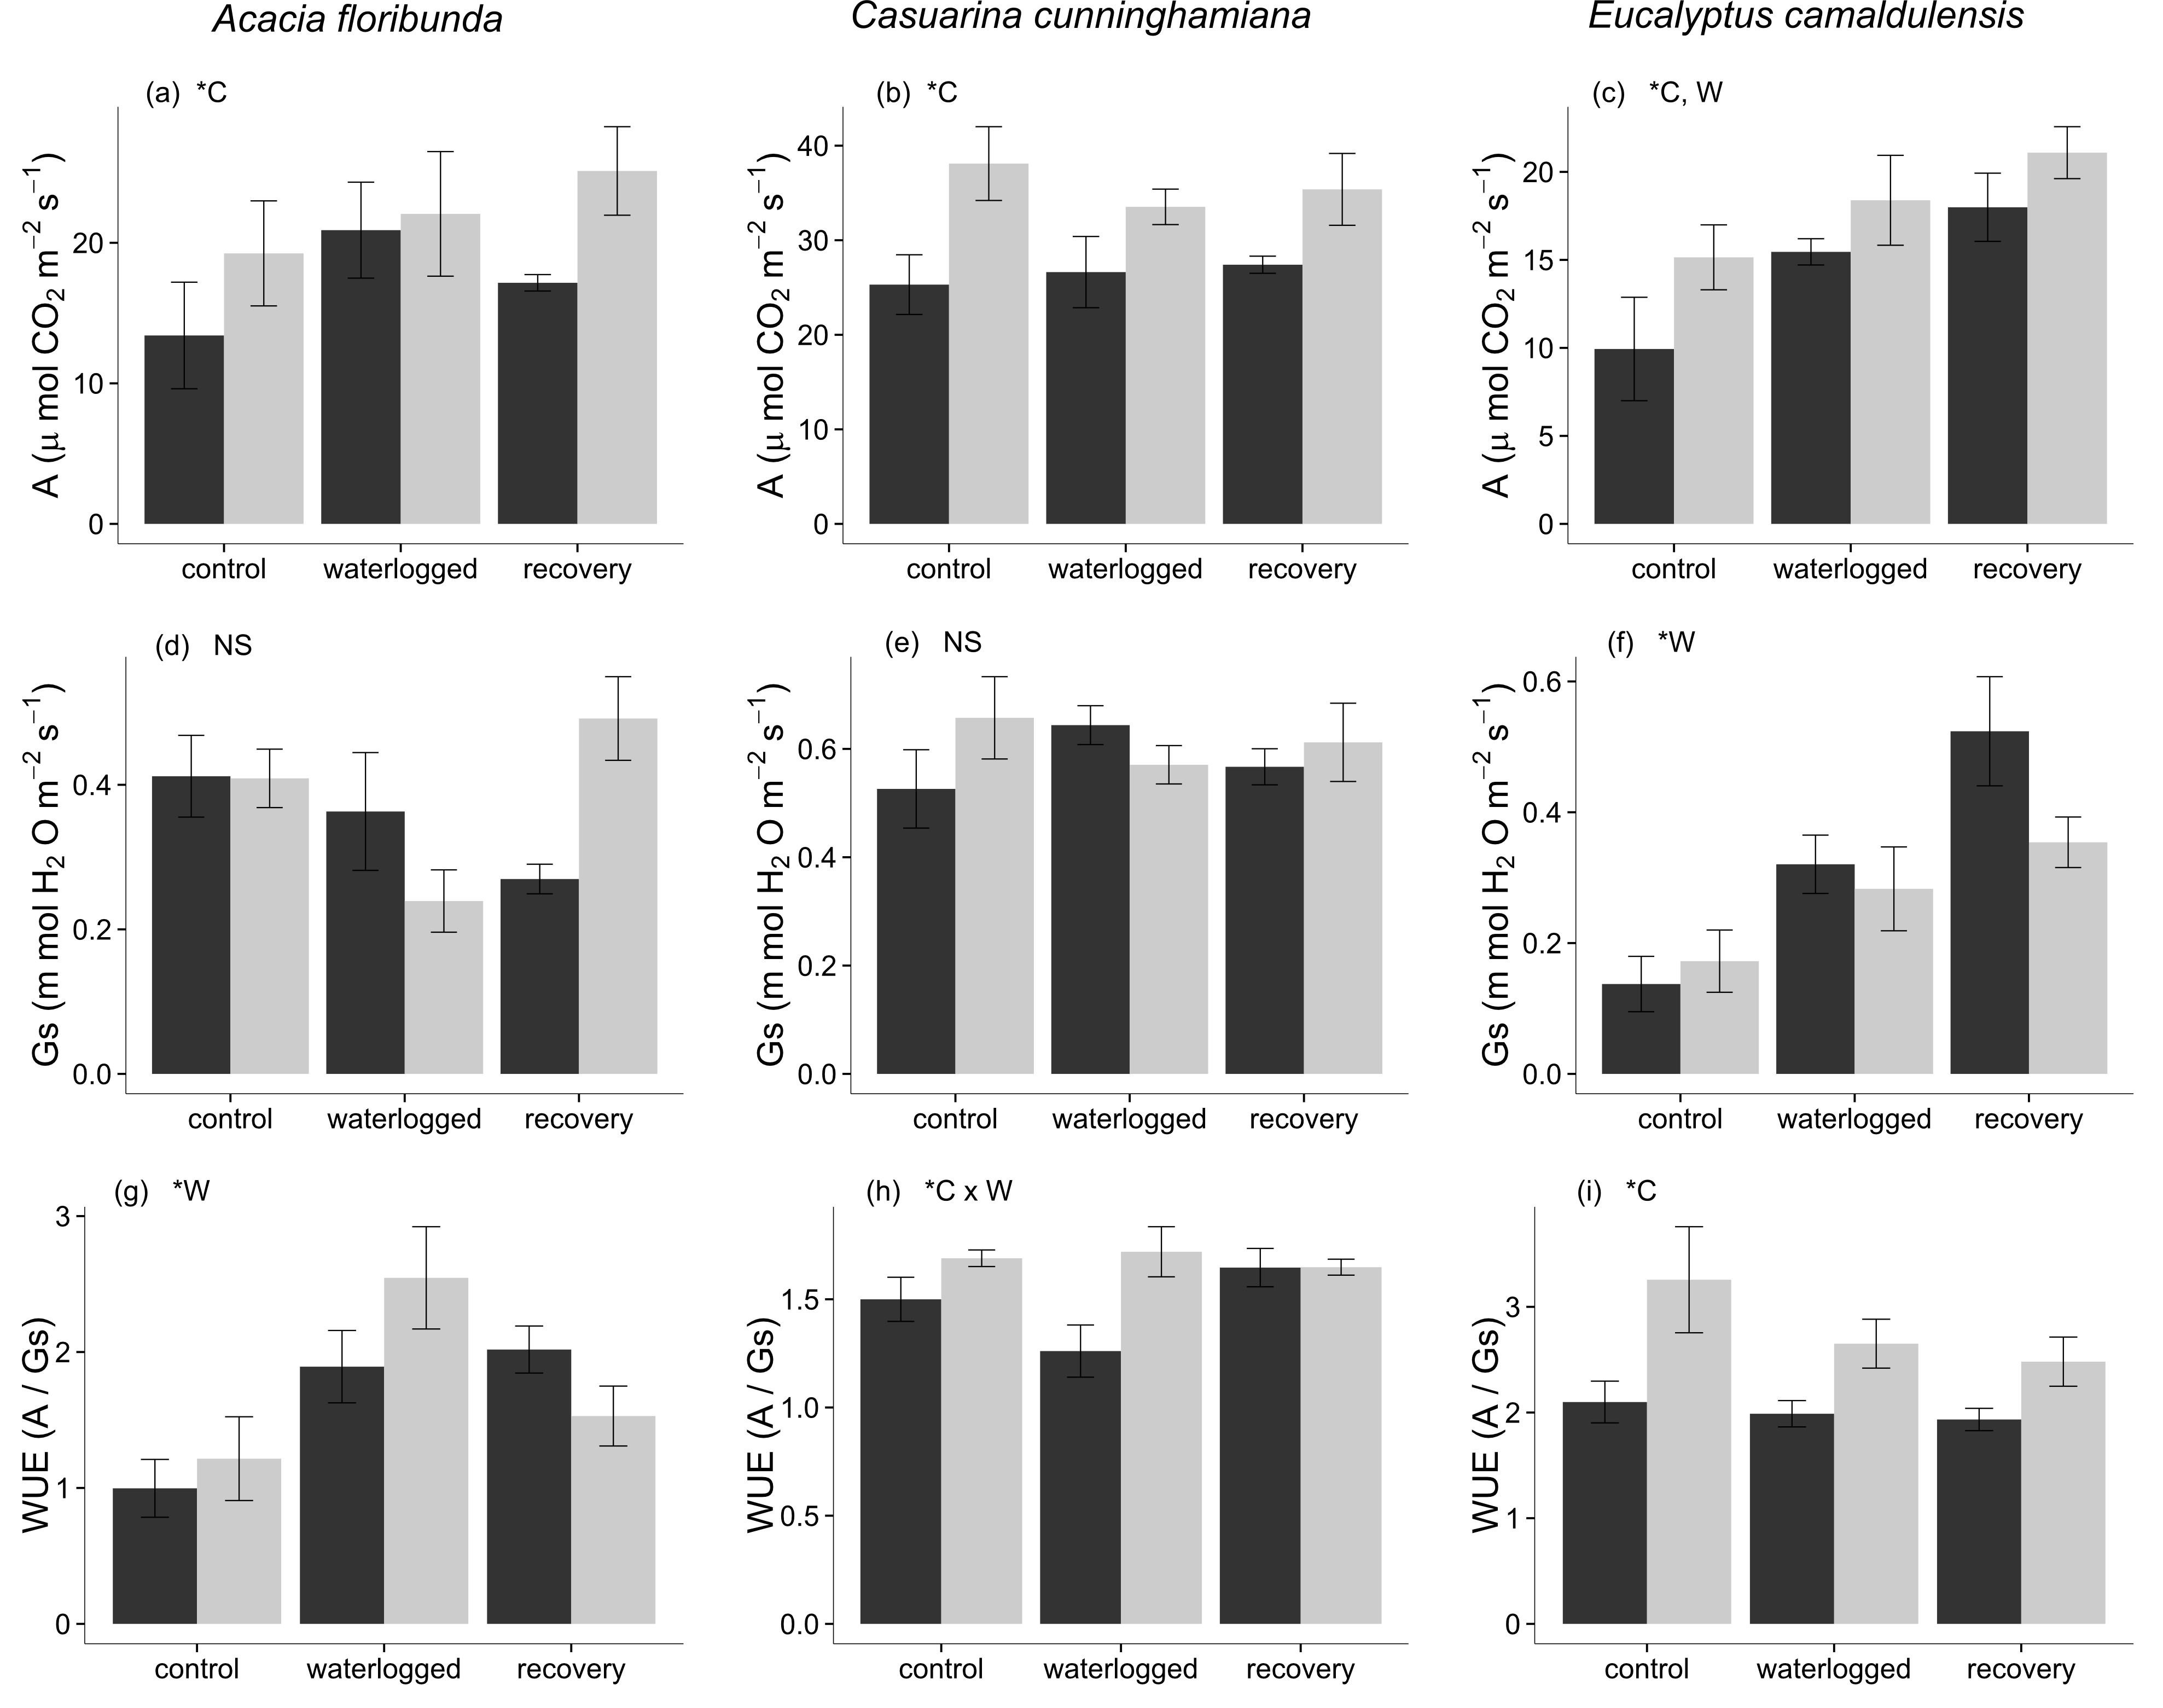
\includegraphics[width=\linewidth,keepaspectratio=true]{gasexchange2.png} % figures can be in pdf, png, jpeg or eps format
\caption[Gas exchange measurements under each combination of waterlogging and CO\textsubscript{2} level treatments.]{\small{Gas exchange measurements under each combination of waterlogging and CO\textsubscript{2} level treatments. Dark shaded columns represent measurements under ambient atmospheric CO\textsubscript{2} concentration (390 ppm), light shaded columns represent measurements under elevated atmospheric CO\textsubscript{2} concentration (550 ppm). Error bars represent the standardised mean error. * - letters denote statistical significance of differences between treatment combinations (NS = no significant difference, C = significant difference between CO\textsubscript{2} level treatments, W = significant difference between waterlogging treatments).}} %The caption in the square bracket is used for the table of figures. The caption in the curved brackets is the one that is printed as actual caption. 
\label{Ch5_F1} % label for cross-referencing
\end{center}
\end{figure}

\subsection*{Biomass production and allocation}
Waterlogging status and CO\textsubscript{2} level interacted strongly for one species: eCO\textsubscript{2} stimulation of all fractions of biomass production in C. cunninghamiana was diminished following recovery from waterlogging. 

Total root biomass of plants recovering from waterlogging was lower than control plants for A. floribunda (p = 0.028, Fig. 2a). A significant interaction effect was identified for C. cunninghamiana (p = 0.049): total root biomass was substantially increased under eCO\textsubscript{2} for control (p = 0.011) but not recovery plants (Fig. 2b). Neither CO\textsubscript{2} level nor waterlogging had an effect on total root biomass for E. camaldulensis (Fig. 2c). 

Fine root biomass of A. floribunda was lower in recovery plants than control plants (p = 0.005), with no CO\textsubscript{2} effect (Fig. 2d). A marginally significant interaction effect was also present for C. cunninghamiana fine root biomass (p = 0.076); post-hoc analysis confirmed that control but not recovery plants had significantly greater fine root biomass under eCO\textsubscript{2} (p = 0.008) (Fig. 2e). Waterlogging stimulated fine root growth in E. camaldulensis (p = 0.046) but CO\textsubscript{2} level had no effect (Fig. 2f).

Neither CO\textsubscript{2} level nor waterlogging had any effect on shoot biomass for A. floribunda (Fig. 2g) or E. camaldulensis (Fig. 2i). As with total root biomass and fine root biomass, CO\textsubscript{2} level and waterlogging influenced C. cunninghamiana biomass interactively (p = 0.009): shoot biomass was higher under eCO\textsubscript{2} for control (p = 0.015) but not recovery plants (Fig. 2h).

Root mass fraction (RMF) was decreased by waterlogging for all species, but no significant CO\textsubscript{2} or interaction effects were found (Fig. 2j-l). RMF of A. floribunda was lower in waterlogged than control plants (p < 0.0001), and lower in waterlogged than recovery plants (p < 0.0001). RMF of A. floribunda recovery plants was also lower than control plants (p = 0.016). RMF of both C. cunninghamiana and E. camaldulensis was lower in waterlogged than control plants (p < 0.0001), and lower in waterlogged than recovery plants (p < 0.0001), but there was no difference between recovery and control plants.

%%%% FIGURE 2
\begin{figure}[h!t]
\begin{center}
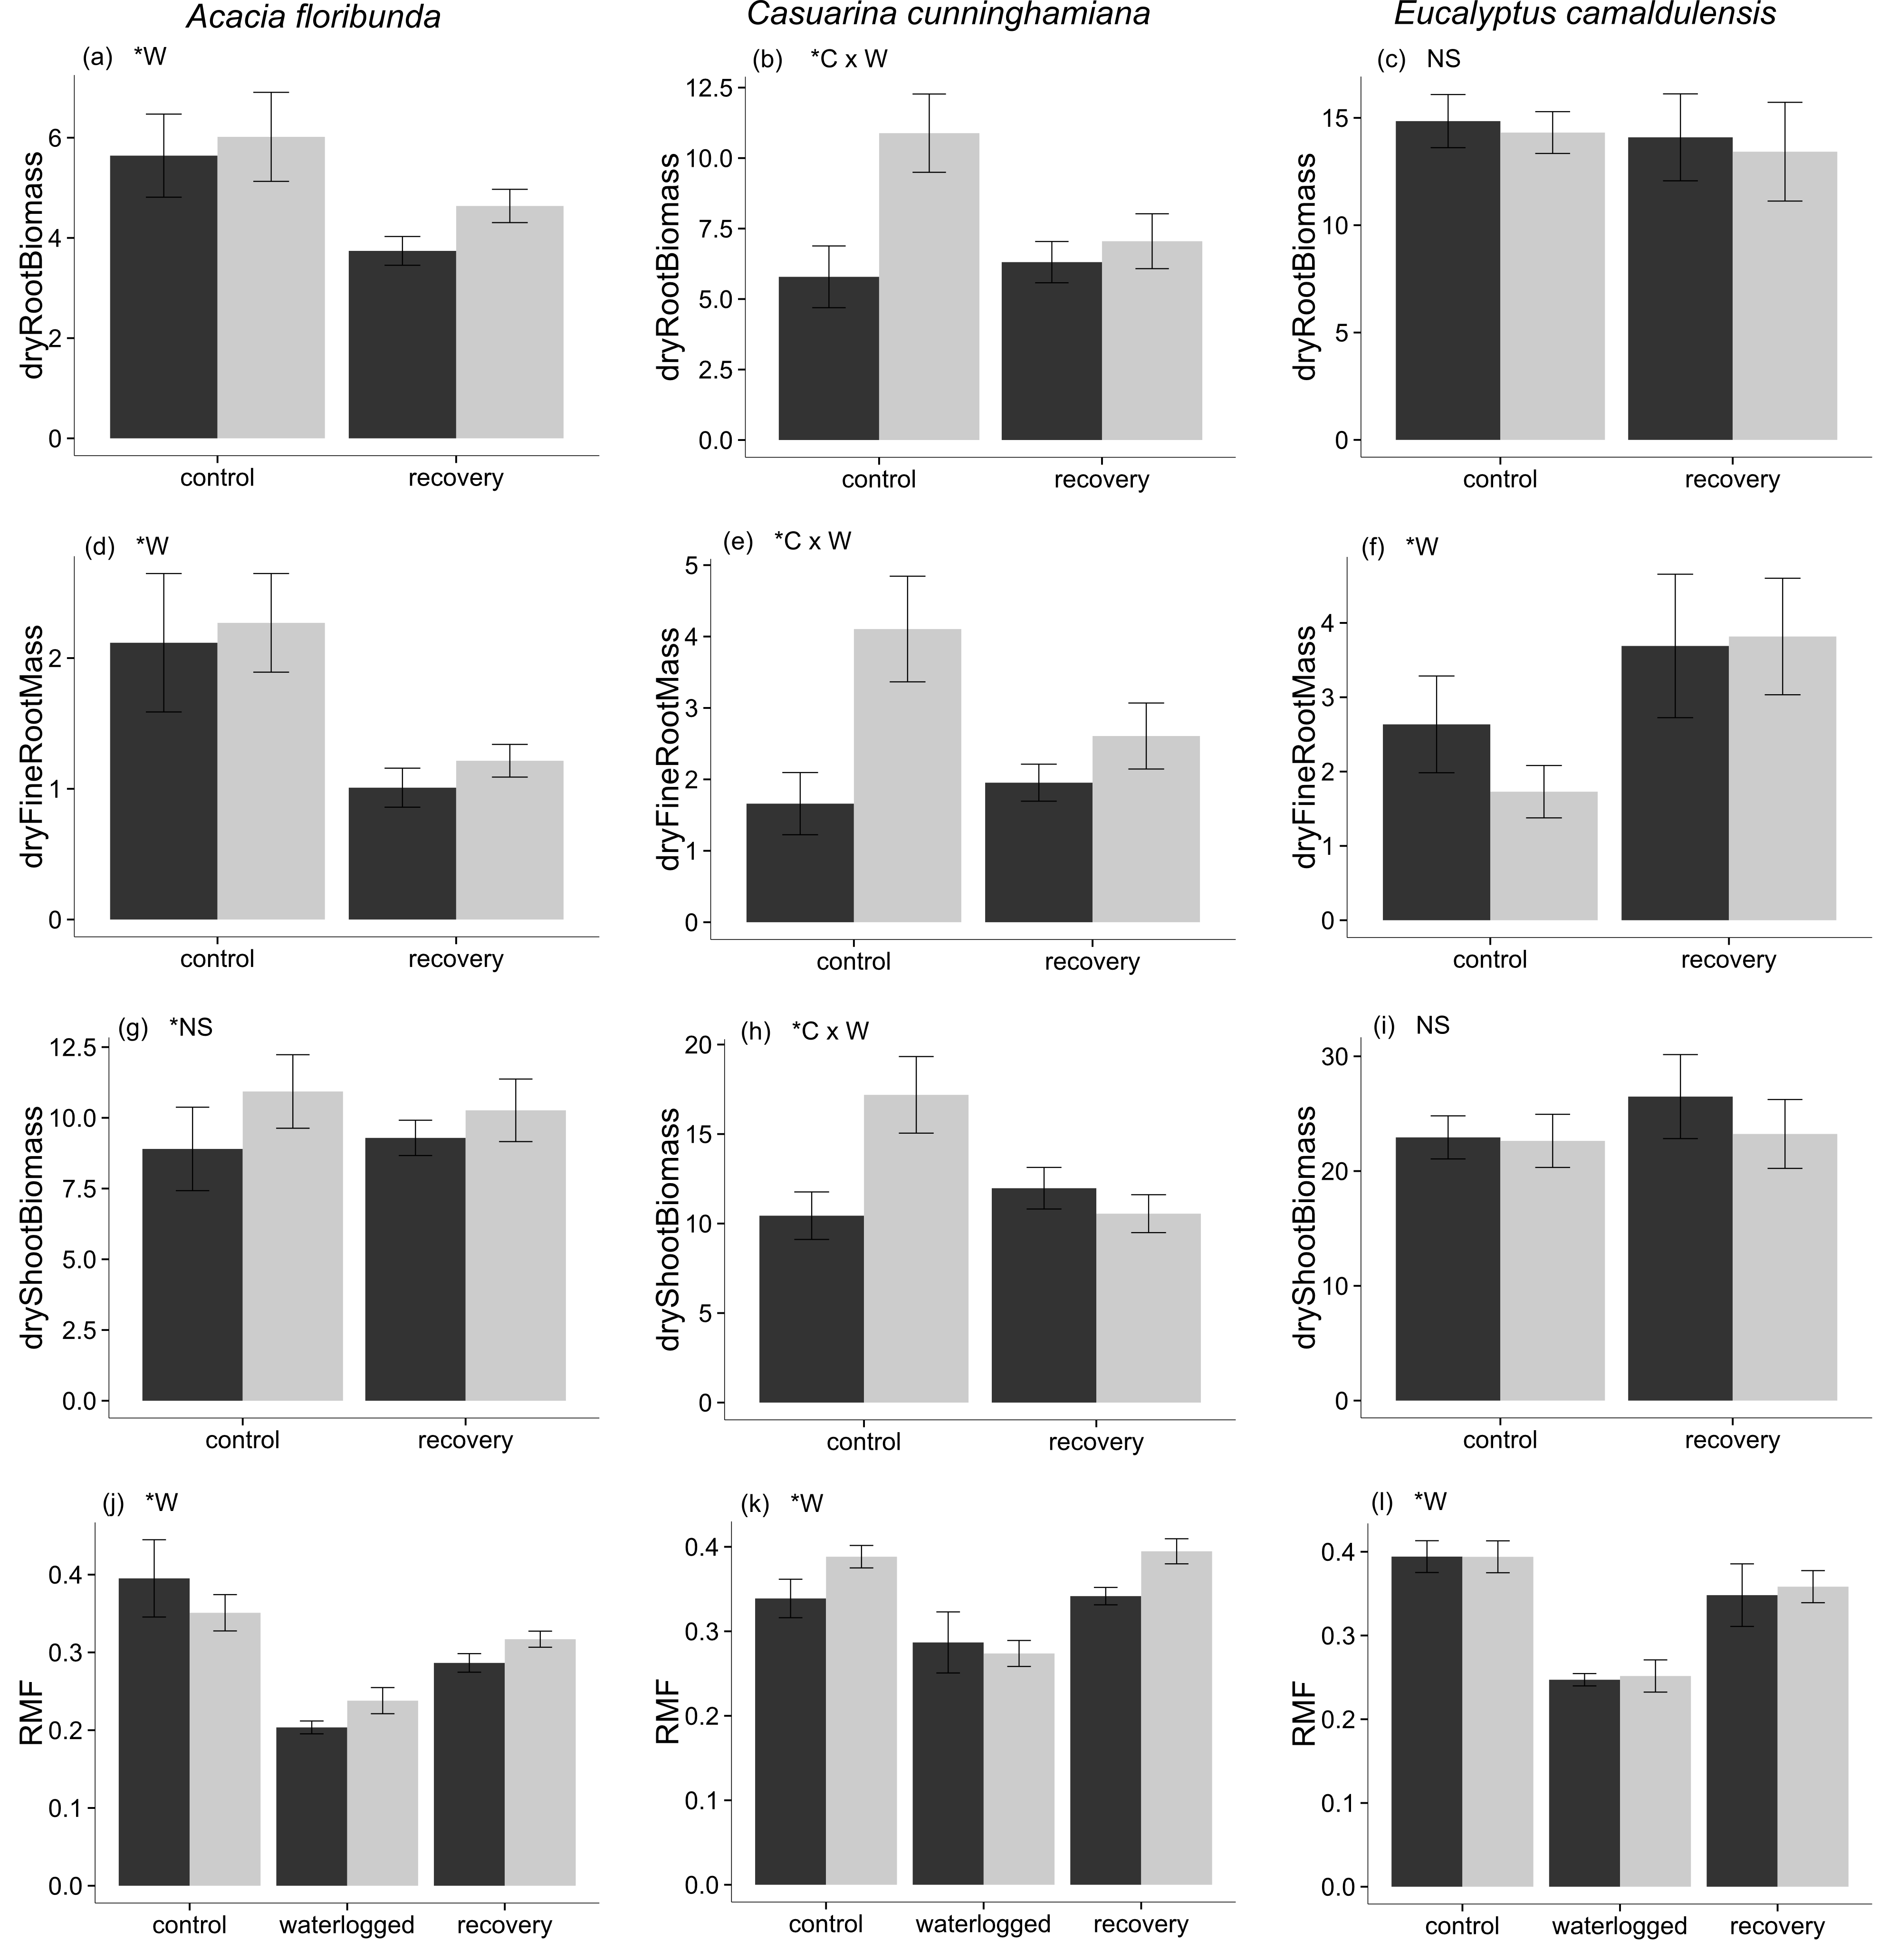
\includegraphics[width=\linewidth, keepaspectratio=true]{biomass2.png} % figures can be in pdf, png, jpeg or eps format
\caption[Biomass and root mass fraction (RMF) measurements under each combination of waterlogging and CO\textsubscript{2} level treatments.]{\small{Biomass and root mass fraction (RMF) measurements under each combination of waterlogging and CO\textsubscript{2} level treatments. Dark shaded columns represent measurements under ambient CO\textsubscript{2} concentration (390 ppm), light shaded columns represent measurements under elevated CO\textsubscript{2} concentration (550 ppm). Error bars represent the standardised meanerror. * - letters denote statistical significance of differences between treatment combinations (NS = no significant difference, C = significant difference between CO\textsubscript{2} level treatments, W = significant difference between waterlogging treatments).}} %The caption in the square bracket is used for the table of figures. The caption in the curved brackets is the one that is printed as actual caption. 
\label{Ch5_F2} % label for cross-referencing
\end{center}
\end{figure}

\subsection*{Functional traits}
We found no evidence to suggest that CO\textsubscript{2} mediates functional traits in response to waterlogging status.

Fine root dry matter content (fRDMC) was higher in waterlogged A. floribunda than recovery plants (p = 0.027), but not different between control and recovery or control and waterlogged plants. A marginally significant interaction effect was also present for A. floribunda (p = 0.067), but no differences were significant upon post-hoc analysis. Waterlogging status also affected E. camaldulensis fRDMC (Fig. 3b): control plants had higher fRDMC than waterlogged plants (p = 0.018), and recovery plants (p = 0.053) (marginally significant). eCO\textsubscript{2} was associated with significantly increased fRDMC in C. cunninghamiana (p = 0.013, Fig. 3c), but waterlogging status had no effect.

Waterlogged A. floribunda had lower SLA than control (p = 0.001), and recovery plants (p < 0.0001) (Fig. 3 d). Waterlogged E. camaldulensis had higher SLA than control (p = 0.0013) and recovery plants (p = 0.0006) (Fig. 3f). Waterlogging status had no effect on C. cunninghamiana SLA (Fig. 3e). CO\textsubscript{2} level had no effect on the SLA of any species. 

Stem density in C. cunninghamiana was increased under elevated CO\textsubscript{2} (p = 0.0177) (Fig. 3h). Stem density was lower in waterlogged C. cunninghamiana than control (p = 0.0167) or recovery plants (0.050) Neither CO\textsubscript{2} nor waterlogging status had any effect on stem density of A. floribunda (Fig. 3g) or E. camaldulensis (3i).

%%%% FIGURE 3
\begin{figure}[h!t]
\begin{center}
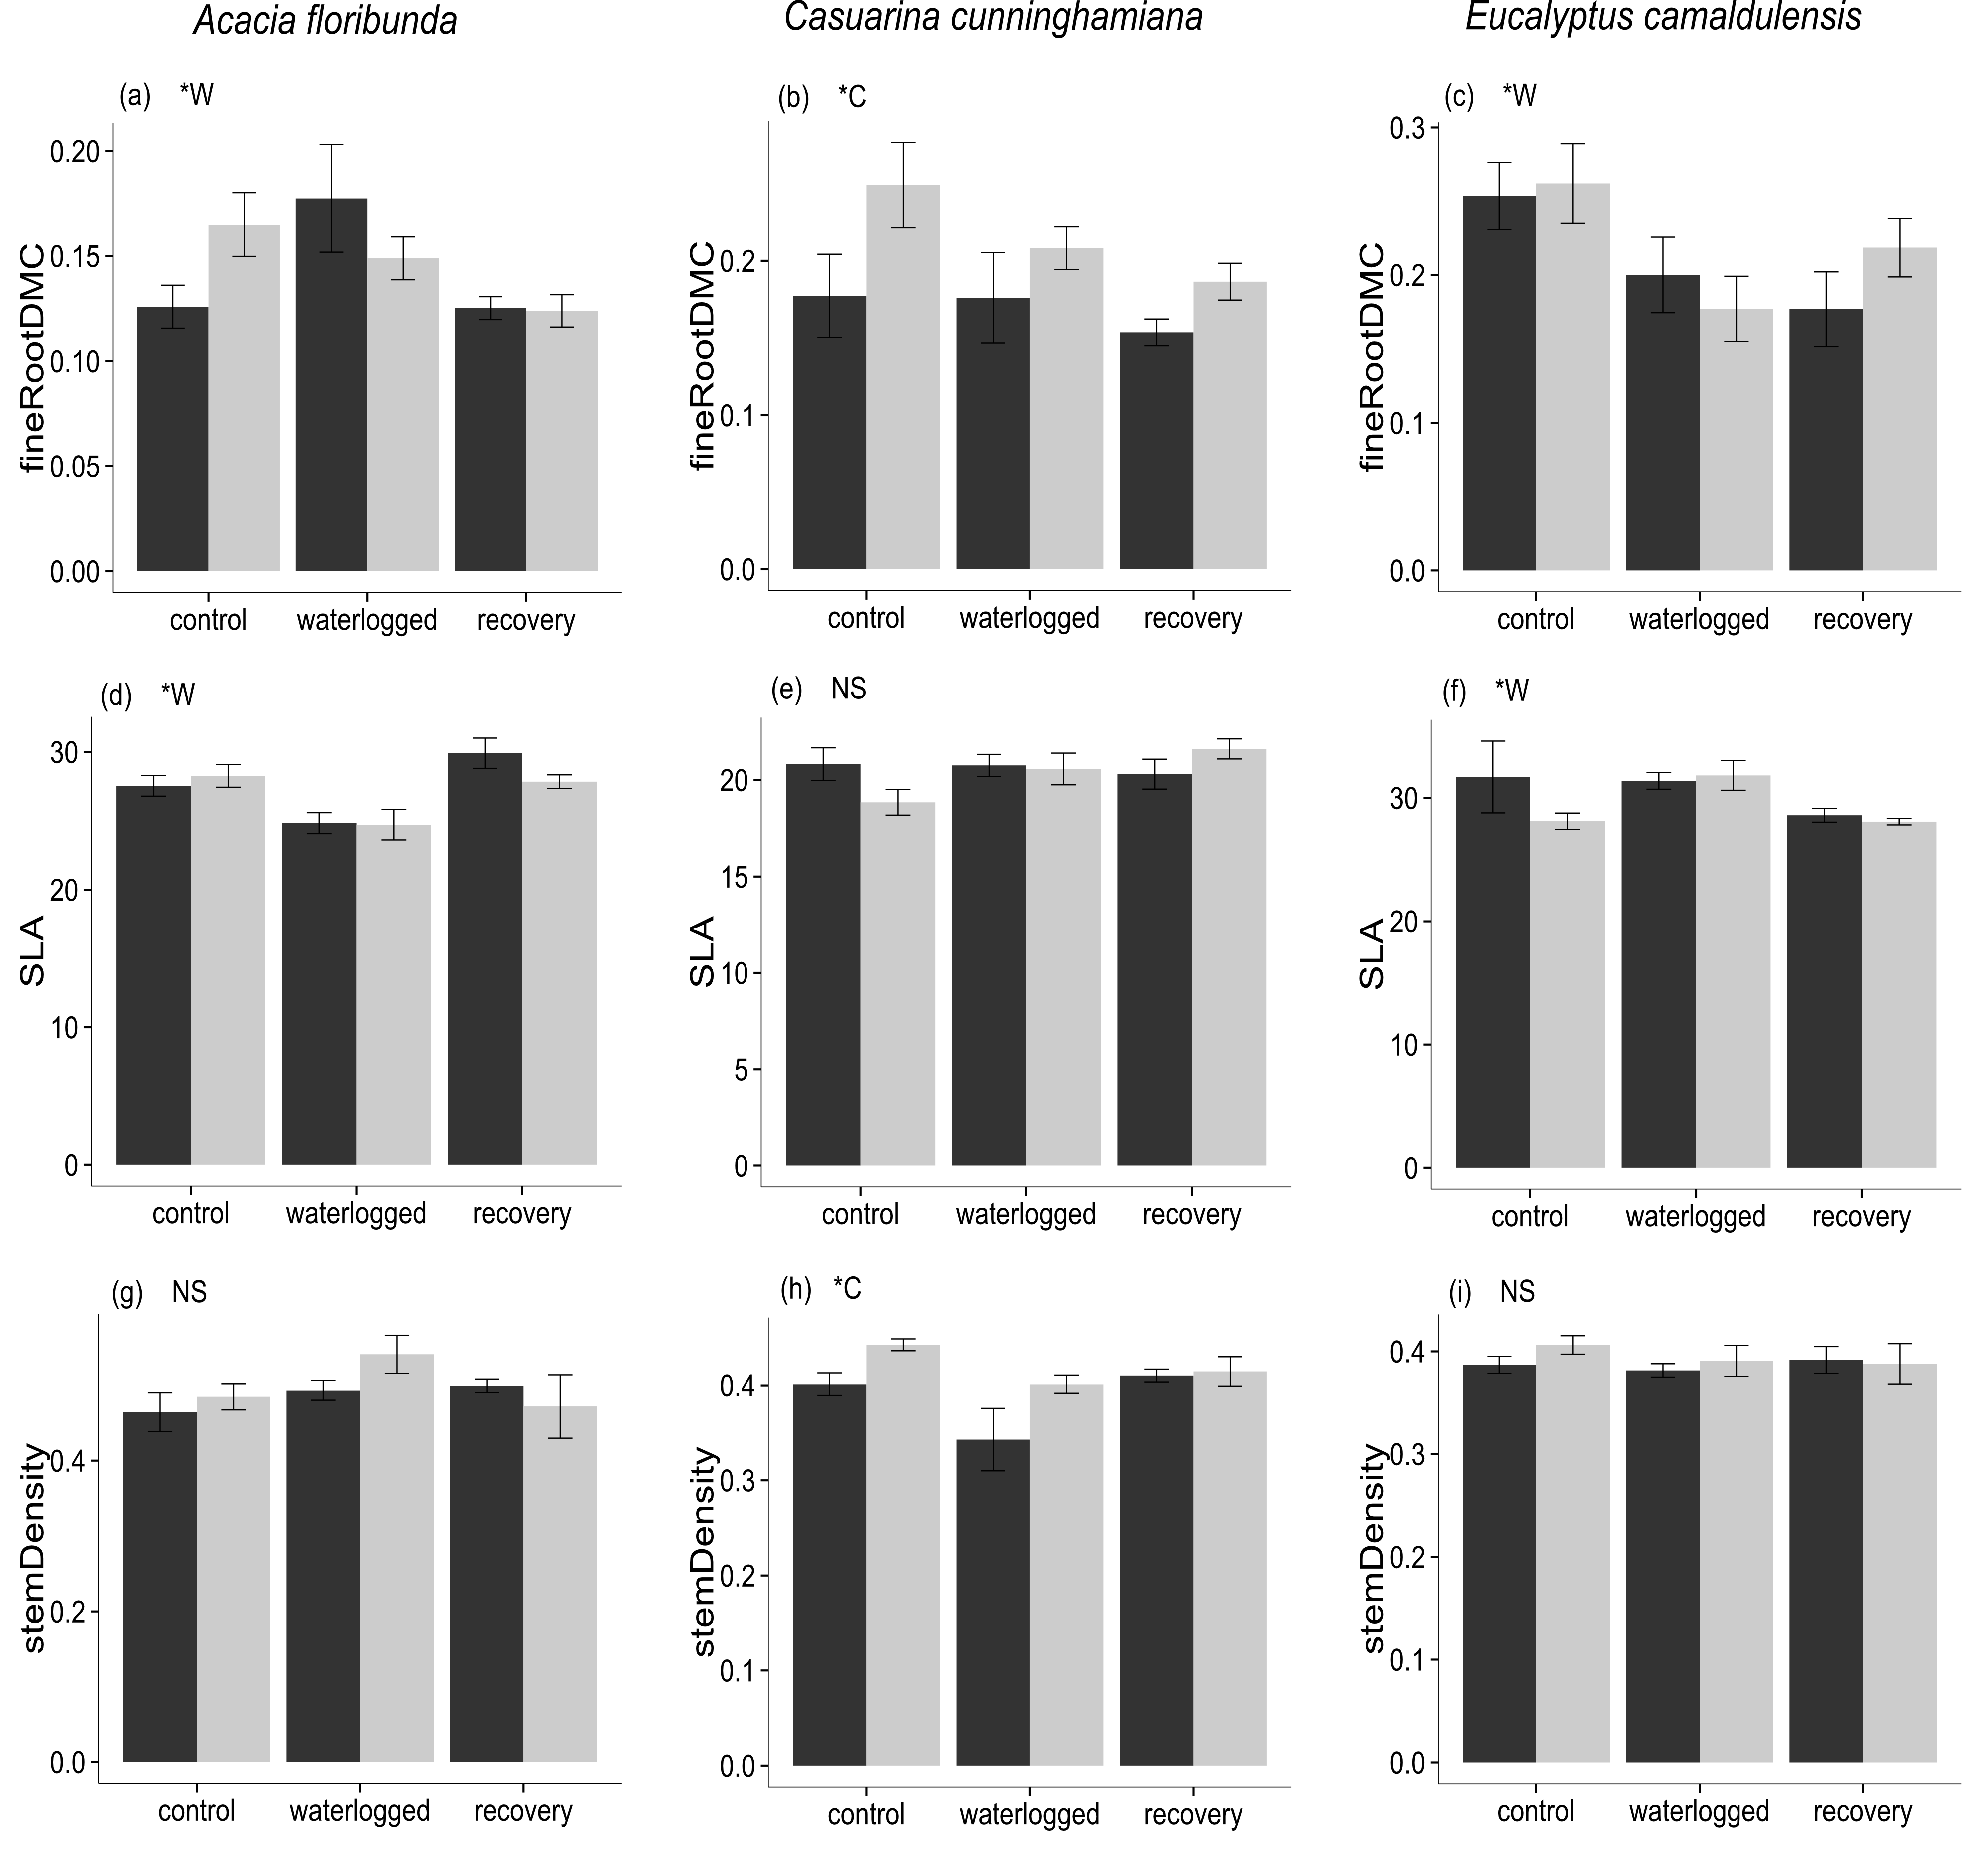
\includegraphics[width=\linewidth,keepaspectratio=true]{traits2.png} % figures can be in pdf, png, jpeg or eps format
\caption[Functional trait measurements under each combination of waterlogging and CO\textsubscript{2} level treatments.]{\small{Functional trait measurements under each combination of waterlogging and CO\textsubscript{2} level treatments. Dark shaded columns represent measurements under ambient CO\textsubscript{2} concentration (390 ppm), light shaded columns represent measurements under elevated CO\textsubscript{2} concentration (550 ppm). Error bars represent the standardised mean error. * - letters denote statistical significance of differences between treatment combinations (NS = no significant difference, C = significant difference between CO\textsubscript{2} level treatments, W = significant difference between waterlogging treatments).}} %The caption in the square bracket is used for the table of figures. The caption in the curved brackets is the one that is printed as actual caption. 
\label{Ch5_F3} % label for cross-referencing
\end{center}
\end{figure}

\section{Discussion}
We found inconsistent effects of atmospheric CO\textsubscript{2} concentration and waterlogging status on growth, gas exchange and functional traits between species of riparian tree seedlings and no evidence for a consistent effect of elevated CO\textsubscript{2} in mediating plant responses to flooding. 

While photosynthesis is the primary means by which plants accumulate biomass, increases in leaf-level photosynthesis may not necessarily translate to biomass gains. Metabolically costly responses to waterlogging tolerance, such as anaerobic catabolism, detoxification of reactive oxygen species and metal ions, and morphological adaptations such as formation of adventitious roots may act as energetic sinks \citep{Colmer2009}. Relationships between photosynthetic rate and biomass responses to waterlogging and CO\textsubscript{2} level treatments in this study varied widely between species.

For the three species studied here, only for C. cunninghamiana was an interactive effect of CO\textsubscript{2} concentration and waterlogging status found. Biomass of shoot, total root and fine root fractions was significantly higher under eCO\textsubscript{2} for control C. cunninghamiana plants, but not for plants which were recovering from waterlogging, despite increased rates of CO\textsubscript{2} assimilation. No significant interaction effect on root mass fraction was found, but visual inspection of the data (Fig. 2k) indicates that eCO\textsubscript{2} stimulation of RMF was present in control and recovering, but not waterlogged plants. Re-establishment of pre-waterlogging biomass allocation appears to have occurred despite no differences in total biomass. We found no evidence to support the hypothesis that eCO\textsubscript{2} facilitated biomass recovery by increasing the rate of fine root production in C. cunninghamiana after waterlogging. Photosynthesis remained higher in recovering plants under eCO\textsubscript{2}, indicating that their ability to convert the extra photosynthate produced under eCO\textsubscript{2} into biomass was impaired by waterlogging. 

No increase in any biomass fraction was associated with increased photosynthetic rate under eCO\textsubscript{2} for either A. floribunda or E. camaldulensis. A. floribunda underwent substantial root mortality in response to waterlogging, although the presence of spongy white aerenchymous adventitious roots indicated a degree of morphological adaptation to anoxia \citep{Evans2004}. Conversely, waterlogging stimulated fine root growth in E. camaldulensis. A proliferation of fine aerenchymous roots both below and above the water line was observed in waterlogged and recovered plants, corresponding to increased fine root mass compared with control plants. The strong morphological response of E. camaldulensis root systems combined with higher photosynthetic rate in recovering compared with control plants, and higher stomatal conductance in waterlogged plants than control or recovering plants, indicates that E. camaldulensis responded favourably to waterlogging in this study. This growth response concurs with the results of previous studies \citep{Sena-Gomes1980, Marcar1993}, although see \citep{Kogawara2006}. No evidence was found to support the hypothesis that higher water use efficiency under eCO\textsubscript{2} might facilitate photosynthesis where waterlogging had caused stomatal closure. WUE was altered by waterlogging only in A. floribunda, and by CO\textsubscript{2} level only in E. camaldulensis. WUE was dependent on the combination of waterlogging status and CO\textsubscript{2} level in C. cunninghamiana, being higher at eCO\textsubscript{2} than aCO\textsubscript{2} for waterlogged plants only. The lack of stomatal response to waterlogging indicates that higher WUE under eCO\textsubscript{2} is not the mechanism maintaining photosynthetic rate under waterlogging for C. cunninghamiana. 

Waterlogging and atmospheric CO\textsubscript{2} level also altered functional traits in a species-specific manner, but no interactive effects were found. Traits of A. floribunda and E. camaldulensis were affected by waterlogging status but not CO\textsubscript{2} level, whereas C. cunninghamiana was affected by CO\textsubscript{2}. Decreased SLA and increased fine root dry matter content – a proxy for fine root tissue density \citep{Birouste2013} – in waterlogged A. floribunda indicate a shift towards the slower growth – longer lifespan  end of their respective economic spectra \citep{Reich2014}, but this shift was not sustained following the refractory period. A corresponding pattern in water use efficiency corroborates this inference. Higher root dry matter content under waterlogging has been linked to the requirement for structural support of air spaces in aerenchymous root tissue \citep{Ryser2011}. Suberization of root hypodermal tissue often occurs under waterlogging as a means of reducing radial oxygen loss \citep{Visser2000, DeSimone2002} and may also increase root dry matter content. E. camaldulensis responded in an opposite manner, with higher SLA under waterlogging, and lower root dry matter content under waterlogging and after the refractory period. This species appears to employ an opportunistic ‘fast growth’ ecological strategy in response to waterlogging, involving proliferation of lower density roots, and lower carbon investment in leaf tissue \citep{Wright2004, Reich2014}. We found no evidence for decreased SLA under eCO\textsubscript{2} as previously described \citep{Poorter2003a}. Previous studies report inconsistent effects of eCO\textsubscript{2} on fine root dry matter content in non-riparian species: eCO\textsubscript{2} had no effect on Liquidambar styraciflua or Pinus strobus fRDMC \citep{Bauer2001,Iversen2008}, caused a small decrease in Betula alleghaniensis \citep{Bauer2001} and increased fRDMC in cotton \citep{Prior1994}. In this study, eCO\textsubscript{2} significantly increased fine root dry matter content in C. cunninghamiana irrespective of waterlogging treatment.

Analysis of gas exchange, biomass accumulation and functional traits after a refractory period provided an opportunity to determine whether responses to waterlogging persisted or were transitory. We were unable to substantiate the hypothesis that eCO\textsubscript{2} would increase the rate of biomass recovery from waterlogging by increasing the rate of fine root turnover. C. cunninghamiana was the only species for which eCO\textsubscript{2} altered biomass accumulation, and depression of biomass was observed following the refractory period irrespective of CO\textsubscript{2} level. Although we made no analysis of nodulation rates, nodulation of C. cunninghamiana by the nitrogen fixing ascomycete Frankia is known to be highest under well aerated soil conditions \citep{Dawson1989}. Reduced nitrogen uptake due to nodule mortality or impairment could account for the constrained biomass response to eCO\textsubscript{2} post-waterlogging \citep{Reich2006}. While eCO\textsubscript{2} did not mitigate growth reduction or mediate changes to functional traits under waterlogging for any species in this glasshouse study, we did observe reduced growth stimulation by eCO\textsubscript{2} in one species. This effect was strong, and evident across all measured biomass fractions. Differential responses to eCO\textsubscript{2} and waterlogging between species in the field could have important ecological consequences. C. cunninghamiana is a highly effective agent of ‘biogeomorphic succession’ in fluvial landscape of south-eastern Australia – that is, it facilitates the creation and stabilisation of fluvial landforms \citep{Erskine2009}. Reduction of eCO\textsubscript{2} biomass stimulation by waterlogging could alter spatial patterns of landform stabilisation by C. cunninghamiana. Infrequently waterlogged stands on channel banks might be favoured over stands growing on wetter in-channel features such as bars, benches and islands. Differential responses to combined waterlogging and eCO\textsubscript{2} between species – notably C. cunninghamiana and A. floribunda, which are frequently conspecific – may also result in compositional changes to riparian plant communities and associated changes in ecosystem functioning.

\section{Conclusion}
Waterlogging and atmospheric CO\textsubscript{2} concentration both have significant consequences for physiological processes, growth and functional characteristics of riparian tree seedlings. The relative importance of these environmental factors varies according to species, as do the specific effects of each on plants. This study adds to the small but growing body of literature describing the interactive effects of waterlogging and CO\textsubscript{2} concentration; notably, the outcome for C. cunninghamiana concurs with that found for Taxodium distichum, a flood tolerant colonist of alluvial riparian areas in the south eastern United States \citep{Megonigal2005}. Blunting of eCO\textsubscript{2} biomass stimulation in seedlings by waterlogging has the potential to alter demographics and structural dynamics in many Australian riparian communities especially where C. cunninghamiana is a keystone species \citep{Woolfrey2001}.

\section*{Acknowledgements}
We would like to thank Urvashi Lallu, Claire Laws, Samiya Tabassum and Daniel Sloane for their help in the glasshouse, and Anthony Manea, Brian Atwell and Melanie Zeppel for providing advice on study design and implementation.

%%%%% REFERENCES % this is in a new chapter due to the memoir format
\renewcommand\bibname{{References}} 
\begin{small}
\bibliographystyle{apalike}
\bibliography{library}
\end{small}
\end{document}

